%%%%%%%%%%%%%%%%%%%%%%%%%%%%%%%%%%%%%%%%%%%%%%%%%%%%%%%%%%%%%%%%%%%%%%%%%%%%%%%%%%
\begin{frame}[fragile]\frametitle{}
\begin{center}
{\Large Reasoning LLMs}

{\tiny (Ref: Reasoning LLMs With a deep dive into DeepSeek-R1 by Dr. Nimrita Koul and more)}

\end{center}


\end{frame}

%%%%%%%%%%%%%%%%%%%%%%%%%%%%%%%%%%%%%%%%%%%%%%%%%%%%%%%%%%%%%%%%%%%%%%%%%%%%%%%%%%
\begin{frame}[fragile]{What is Reasoning?}
    \begin{itemize}
        \item Reasoning is the ability to draw conclusions based on facts, rules or evidence
		\item Types:
			    \begin{itemize}
				\item  Deductive: ``All humans are mortals, I am a human, so I am mortal. ''
				\item  Inductive: Inferring general patterns from specific examples. `` The sun has risen in the east every day I have observed. The sun will rise in the east tomorrow as well. ''
				\item  Abductive: Making educated guesses e.g. diagnosis from symptoms.
				\item  Probabilistic: Bayesian Inference.
			\end{itemize}
    \end{itemize}
\end{frame}

%%%%%%%%%%%%%%%%%%%%%%%%%%%%%%%%%%%%%%%%%%%%%%%%%%%%%%%%%%%%%%%%%%%%%%%%%%%%%%%%%%
\begin{frame}[fragile]{What is Logical Reasoning?}
    \begin{block}{Logical Reasoning}
		A farmer is going to the market with a wolf, a goat, 
		and a cabbage. He comes to a river with a small boat 
		that can carry only him and one of the three items at 
		a time. If left alone together, the wolf will eat the goat, 
		and the goat will eat the cabbage. How can the 
		farmer get everything safely across the river?
    \end{block}
\end{frame}

%%%%%%%%%%%%%%%%%%%%%%%%%%%%%%%%%%%%%%%%%%%%%%%%%%%%%%%%%%%%%%%%%%%%%%%%%%%%%%%%%%
\begin{frame}[fragile]{What is Mathematical Reasoning?}
    \begin{block}{Mathematical Reasoning}
		 A shopkeeper sells an item at a 20\% profit. If the 
		cost price of the item is increased by Rs 50 and the 
		selling price remains the same, the profit 
		percentage drops to 10\%. What is the original cost 
		price of the item?
    \end{block}
\end{frame}

%%%%%%%%%%%%%%%%%%%%%%%%%%%%%%%%%%%%%%%%%%%%%%%%%%%%%%%%%%%%%%%%%%%%%%%%%%%%%%%%%%
\begin{frame}[fragile]{What is AI Reasoning?}
    \begin{itemize}
        \item AI Algorithms can reason using strict logic rules (rule-based systems)or using flexible 
pattern recognition from input data (neural networks). 
        \item Reasoning models can accurately solve verifiable tasks—such as math, logic puzzles and coding 
tasks.
        \item Models like Anthropic's Claude 3.7 Sonnet, OpenAI's o1, o3, and DeepSeek's DeepSeek- R1 
are reasoning LLMs. 
        \item Such reasoning LLMs are built by finetuning large base models using Reinforcement Learning.
    \end{itemize}
\end{frame}

%%%%%%%%%%%%%%%%%%%%%%%%%%%%%%%%%%%%%%%%%%%%%%%%%%%%%%%%%%%%%%%%%%%%%%%%%%%%%%%%%%
\begin{frame}[fragile]{Training: Existing: ChatGPT}
    \begin{itemize}
        \item Pretraining 
        \item Supervised Finetuning (SFT)
        \item Reinforcement Learning through Human Feedback (RLHF)
    \end{itemize}
\end{frame}

%%%%%%%%%%%%%%%%%%%%%%%%%%%%%%%%%%%%%%%%%%%%%%%%%%%%%%%%%%%%%%%%%%%%%%%%%%%%%%%%%%
\begin{frame}[fragile]{Inference}

Inference Time Strategies to build Reasoning Capabilities 

    \begin{itemize}
        \item  Chain of Thought: Long CoT allows LLMs to generate more tokens and multiple outputs thus spending more computation power on a problem during inference. 
        \item  With Long Chain of Thought (LongCoT) prompting LLMs is made to generate a series of intermediate reasoning steps before giving a final answer. 
        \item  The prompt ``Let's think this through step by step'' enables reasoning.
    \end{itemize}
\end{frame}


%%%%%%%%%%%%%%%%%%%%%%%%%%%%%%%%%%%%%%%%%%%%%%%%%%%%%%%%%%%%%%%%%%%%%%%%%%%%%%%%%%
\begin{frame}[fragile]\frametitle{Chain of Thoughts}
		\begin{center}
		\includegraphics[width=\linewidth,keepaspectratio]{promptengg25}
		\end{center}

\end{frame}


%%%%%%%%%%%%%%%%%%%%%%%%%%%%%%%%%%%%%%%%%%%%%%%%%%%%%%%%%%%%%%%%%%%%%%%%%%%%%%%%%%
\begin{frame}[fragile]{Long vs Standard CoT}


    \begin{itemize}
        \item  standard CoT is short and human-readable, a long CoT is several thousand tokens long  and not very human readable. 
		\item  long and complex reasoning trace behaviors
    \end{itemize}
\end{frame}

%%%%%%%%%%%%%%%%%%%%%%%%%%%%%%%%%%%%%%%%%%%%%%%%%%%%%%%%%%%%%%%%%%%%%%%%%%%%%%%%%%
\begin{frame}[fragile]{Parallel Decoding}


    \begin{itemize}
        \item   Instead of generating a single output with LLM, it generates multiple 
outputs and aggregates these outputs to form a single, final answer. 
    \end{itemize}
\end{frame}

%%%%%%%%%%%%%%%%%%%%%%%%%%%%%%%%%%%%%%%%%%%%%%%%%%%%%%%%%%%%%%%%%%%%%%%%%%%%%%%%%%
\begin{frame}[fragile]{AI Planning}


    \begin{itemize}
        \item AI planning is the search for a sequence of good actions to take to 
achieve a goal (maximize a reward)
\item  Classical AI Planning: solves problems by searching for an action sequence that 
transforms an initial state into a goal state. However, it depends on a correct action models, 
it may not be appropriate for LLMs
\item Reinforcement Learning AI Planning: 
	    \begin{itemize}
        \item to learn a correct sequence of decisions to 
take by interacting with an environment and receiving feedback in the 
form of rewards. 
		\item Over time, the agent learns a policy that maximizes cumulative reward 
(generates best LLM output).  
		\item DeepSeek demonstrated that reinforcement learning can drive complex reasoning improvements in AI without requiring vast supervised datasets.
		\end{itemize}

    \end{itemize}
\end{frame}

%%%%%%%%%%%%%%%%%%%%%%%%%%%%%%%%%%%%%%%%%%%%%%%%%%%%%%%%%%%%%%%%%%%%%%%%%%%%%%%%%%
\begin{frame}[fragile]\frametitle{What is Reinforcement Learning?}
		\begin{center}
		\includegraphics[width=\linewidth,keepaspectratio]{rl1}
		\end{center}

\end{frame}


%%%%%%%%%%%%%%%%%%%%%%%%%%%%%%%%%%%%%%%%%%%%%%%%%%%%%%%%%%%%%%%%%%%%%%%%%%%%%%%%%%
\begin{frame}[fragile]{Use of RL in LLMs}


    \begin{itemize}
        \item  RLHF to fine tune a model
		\item RL to train an AI agent that uses an LLM as part of its decision process.
		\item An LLM agent acting in a simulated environment (say, a text-based 
game or a web navigation task) can be improved via RL by trying actions, 
seeing outcomes, and learning a policy. 
		\item However, pure RL can be sample-inefficient (requiring many trials) and 
lacks guarantees of optimality. Modern techniques like model-based RL 
explicitly learn a model of the environment and plan within it, blending 
classical planning ideas with reinforcement learning.
    \end{itemize}
\end{frame}


%%%%%%%%%%%%%%%%%%%%%%%%%%%%%%%%%%%%%%%%%%%%%%%%%%%%%%%%%%%%%%%%%%%%%%%%%%%%%%%%%%
\begin{frame}[fragile]{To Enhance Reasoning}


    \begin{itemize}
        \item  Chain-of-Thought (CoT) Prompting and Integration
        \item  Enhanced RLHF Integration
        \item  Deliberative Alignment
        \item  Train on Math and Code Combined to  Enhance Model Reasoning
        \item  Reinforcement Learning-Based Reasoning
        \item  Distillation of Large Model Reasoning into Smaller Models
    \end{itemize}
\end{frame}

%%%%%%%%%%%%%%%%%%%%%%%%%%%%%%%%%%%%%%%%%%%%%%%%%%%%%%%%%%%%%%%%%%%%%%%%%%%%%%%%%%
\begin{frame}[fragile]\frametitle{}
\begin{center}
{\Large DeepSeek R1}

{\tiny (Ref: Reasoning LLMs With a deep dive into DeepSeek-R1 by Dr. Nimrita Koul and more)}

\end{center}


\end{frame}



%%%%%%%%%%%%%%%%%%%%%%%%%%%%%%%%%%%%%%%%%%%%%%%%%%%%%%%%%%%%%%%%%%%%%%%%%%%%%%%%%%
\begin{frame}[fragile]{DeepSeek R1 Model Architecture}


    \begin{itemize}
        \item  DeepSeek –R1-Zero and DeepSeek-R1 reasoning models are based on a 
powerful, open-source base model called DeepSeek-v3
        \item  DeepSeek-v3 is a 671 Billion parameter Mixture-of-Experts (MoE) open-
source model . 
        \item  The total size of DeepSeek-V3 models on Hugging Face is 685B, which 
includes 671B of the Main Model weights and 14B of the Multi-Token 
Prediction (MTP) Module weights.
		\item DeepSeek R1 matches the performance of OpenAI's o1 model. 
    \end{itemize}
\end{frame}

%%%%%%%%%%%%%%%%%%%%%%%%%%%%%%%%%%%%%%%%%%%%%%%%%%%%%%%%%%%%%%%%%%%%%%%%%%%%%%%%%%
\begin{frame}[fragile]{DeepSeek-R1-Zero}


    \begin{itemize}
        \item  DeepSeek-R1-Zero is the first reasoning model from DeepSeek.  
DeepSeek-R1-Zero's training strategy uses pure large-scale RL without 
Supervised Fine-tuning. 
        \item  The model self-evolves and learns to use long CoT to solve complex 
reasoning problems through RL
    \end{itemize}
\end{frame}

%%%%%%%%%%%%%%%%%%%%%%%%%%%%%%%%%%%%%%%%%%%%%%%%%%%%%%%%%%%%%%%%%%%%%%%%%%%%%%%%%%
\begin{frame}[fragile]{DeepSeek-R1-Zero Training}

RL with Group Relative Policy Optimization (GRPO)

    \begin{itemize}
        \item  To train DeepSeek-R1-Zero, the DeepSeek-v3 base model is fine-tuned 
directly using RL algorithm called Group Relative Policy Optimization 
(GRPO). GRPO does not need a neural reward model (value function).
        \item   DeepSeek-R1-Zero uses a rules-based reward system 
		\item Training uses two types of rewards:
		    \begin{itemize}
				\item   Accuracy Reward evaluates whether the model's response is correct.
				\item   Format Reward  enforces a desired format on the model's output.  
		    \end{itemize}

    \end{itemize}
\end{frame}

%%%%%%%%%%%%%%%%%%%%%%%%%%%%%%%%%%%%%%%%%%%%%%%%%%%%%%%%%%%%%%%%%%%%%%%%%%%%%%%%%%
\begin{frame}[fragile]{GRPO}


    \begin{itemize}
        \item   GRPO is an RL algo used to train reasoning LLMs. 
        \item   While PPO uses a neural reward model (value function) to estimate 
rewards, GPRO generates multiple responses for each input prompt and 
uses the average reward of these groups of responses as a baseline.  
        \item   Uses KL divergence between current policy and a reference policy (a 
SFT model) into the loss function to ensure stable updates to policy.
        \item   GRPO needs less memory, compute, is stable and scalable. 
    \end{itemize}
\end{frame}


%%%%%%%%%%%%%%%%%%%%%%%%%%%%%%%%%%%%%%%%%%%%%%%%%%%%%%%%%%%%%%%%%%%%%%%%%%%%%%%%%%
\begin{frame}[fragile]{Reward Computation in GRPO}


    \begin{itemize}
        \item    Given a single input, model generates a group/batch of outputs
        \item    A pre-trained reward model trained on preference data is used to assign a 
reward to each output
        \item    Unlike PPO which computes an absolute reward, GRPO computes 
advantage of each response relative to other responses in the same batch. 
The average reward for the batch acts as the baseline for advantage estimation.
        \item     Then GRPO updates the policy using these relative advantages ensuring the 
responses with higher rewards are reinforced. KL divergence is the part of 
objective function to keep the policy close to a reference SFT model. 
    \end{itemize}
\end{frame}

%%%%%%%%%%%%%%%%%%%%%%%%%%%%%%%%%%%%%%%%%%%%%%%%%%%%%%%%%%%%%%%%%%%%%%%%%%%%%%%%%%
\begin{frame}[fragile]{Verifiable Rewards}


    \begin{itemize}
        \item   Using RL to learn from Verifiable Rewards
        \item    We can directly use the verification result (result of string matching 
or code passing test cases) as a reward signal for training with RL. 
        \item   This is the fundamental concept upon which all modern reasoning 
models are based.
        \item    This can be implemented as process rewards or pure RL. 
    \end{itemize}
\end{frame}

%%%%%%%%%%%%%%%%%%%%%%%%%%%%%%%%%%%%%%%%%%%%%%%%%%%%%%%%%%%%%%%%%%%%%%%%%%%%%%%%%%
\begin{frame}[fragile]\frametitle{ Verifiable Rewards}
		\begin{center}
		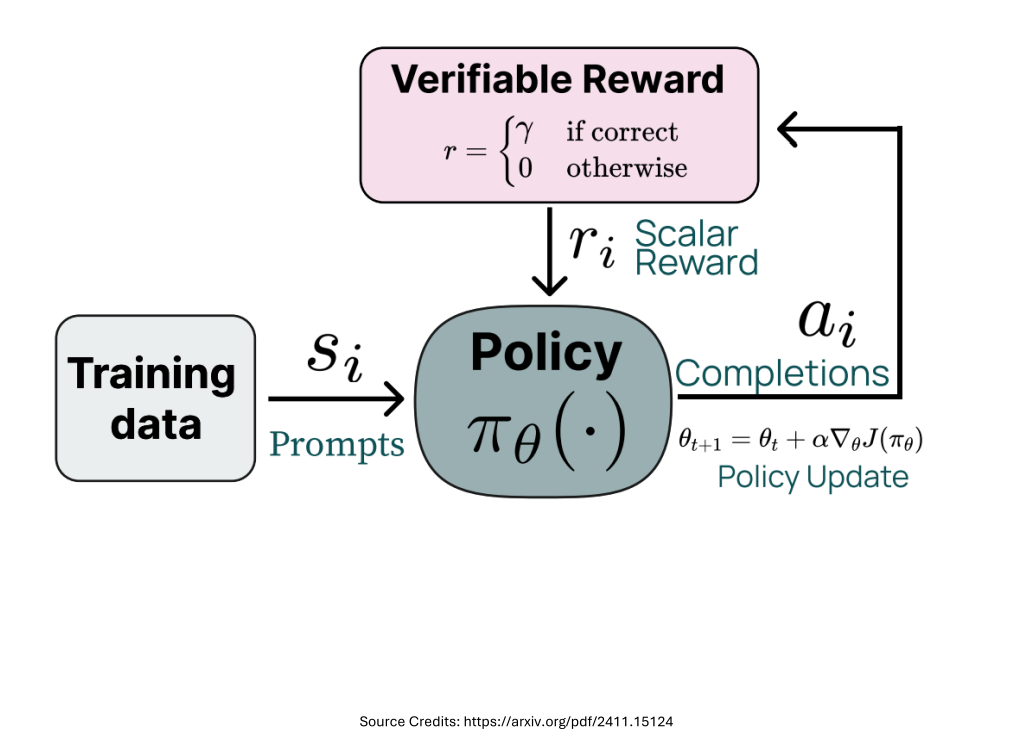
\includegraphics[width=\linewidth,keepaspectratio]{deepseek2}
		\end{center}

\end{frame}

%%%%%%%%%%%%%%%%%%%%%%%%%%%%%%%%%%%%%%%%%%%%%%%%%%%%%%%%%%%%%%%%%%%%%%%%%%%%%%%%%%
\begin{frame}[fragile]{Self-Evolution}

Self-Evolution in DeepSeek-R1-Zero

    \begin{itemize}
        \item    Model was not explicitly taught to decompose problems, search for a 
solution, perform backtracking or evaluate its own line of thought. 
        \item   The LLM autonomously learned necessary behaviours for solving 
problems via an RL-based ``self-evolution'' process. 
    \end{itemize}
\end{frame}

%%%%%%%%%%%%%%%%%%%%%%%%%%%%%%%%%%%%%%%%%%%%%%%%%%%%%%%%%%%%%%%%%%%%%%%%%%%%%%%%%%
\begin{frame}[fragile]{Comparison}

DeepSeek-R1 vs DeepSeek-R1-Zero

    \begin{itemize}
        \item    DeepSeek-R1 differs from DeepSeek-R1-Zero in the addition of a 
language consistency reward which is calculated as the portion of the 
models output written in the desired target language. 
        \item    i.e. While DeepSeek-R1-Zero is good at reasoning, DeepSeek-R1 is good 
at reasoning as well as at generating natural language.
    \end{itemize}
\end{frame}


%%%%%%%%%%%%%%%%%%%%%%%%%%%%%%%%%%%%%%%%%%%%%%%%%%%%%%%%%%%%%%%%%%%%%%%%%%%%%%%%%%
\begin{frame}[fragile]{ Training Pipeline}

DeepSeek-R1's Multistage Training Pipeline

    \begin{itemize}
        \item     Like DeepSeek-R1-Zero, DeepSeek-R1 begins with DeepSeek-v3 as a 
base model. 
        \item     Then, DeepSeek-R1 undergoes four stages of training – 2 steps of SFT 
and 2 steps of RL
    \end{itemize}
\end{frame}

%%%%%%%%%%%%%%%%%%%%%%%%%%%%%%%%%%%%%%%%%%%%%%%%%%%%%%%%%%%%%%%%%%%%%%%%%%%%%%%%%%
\begin{frame}[fragile]{ Stages}



    \begin{itemize}
        \item   Stage One: SFT on Cold Start Data:  During this stage, R1 is trained on a small data set of pairs of prompts and the summaries of their corresponding long CoT reasoning (Supervised Cold Start Data) 
		\item Stage Two: Reasoning Oriented RL: In stage 2, large scale RL is used with additional reward for language consistency.  This language consistency reward improves the overall alignment of 
the resulting model with human preferences – making it more fluent 
and readable. 
		\item Stage Three: SFT on Diverse Data Examples:  In stage 3, another level of SFT is carried out on more diverse dataset. The SFT dataset for the stage 3contained 600K prompt-reasoning trails 
plus 200K non-reasoning prompt-response pairs.
		\item Stage Four: General-purpose RLHF:  In stage 4, RLHF is performed to align the model with human 
preferences. 
    \end{itemize}
\end{frame}


%%%%%%%%%%%%%%%%%%%%%%%%%%%%%%%%%%%%%%%%%%%%%%%%%%%%%%%%%%%%%%%%%%%%%%%%%%%%%%%%%%
\begin{frame}[fragile]{ Architectural Innovations}

Innovations in DeepSeek V3 that make it very economical

    \begin{itemize}
        \item   Use of multi-headed latent attention for better memory footprint
        \item   Use of fine-grained and shared experts in an optimized Mixture of Experts 
structure.
        \item   Use of multi-token prediction objective
        \item   Innovative Load Balancing Strategy and Training Objective
        \item   Uses a reduced FP8 precision throughout training by using a new quantized training 
strategy.
    \end{itemize}
\end{frame}


%%%%%%%%%%%%%%%%%%%%%%%%%%%%%%%%%%%%%%%%%%%%%%%%%%%%%%%%%%%%%%%%%%%%%%%%%%%%%%%%%%
\begin{frame}[fragile]{ Distilled Models}

Distilled Models from DeepSeek-R1

    \begin{itemize}
        \item   To create distilled models – the authors of DeepSeek-R1 began with two 
base models Qwen-2.5  and LLaMA-3. Then the base models were trained 
via SFT over 800K supervised training examples curated in 3 rd  stage of 
training pipeline for DeepSeek-R1. 
        \item  6 models were distilled from DeepSeek-R1 based on Qwen-2.5 and 
LLaMA-3 - (DeepSeek-R1 1.5B, DeepSeek-R1 7B, DeepSeek-R1 8B, 
DeepSeek-R1 14B, DeepSeek-R1 32B, DeepSeek-R1 70B)
    \end{itemize}
\end{frame}


%%%%%%%%%%%%%%%%%%%%%%%%%%%%%%%%%%%%%%%%%%%%%%%%%%%%%%%%%%%%%%%%%%%%%%%%%%%%%%%%%%
\begin{frame}[fragile]\frametitle{ Performance Comparison}
		\begin{center}
		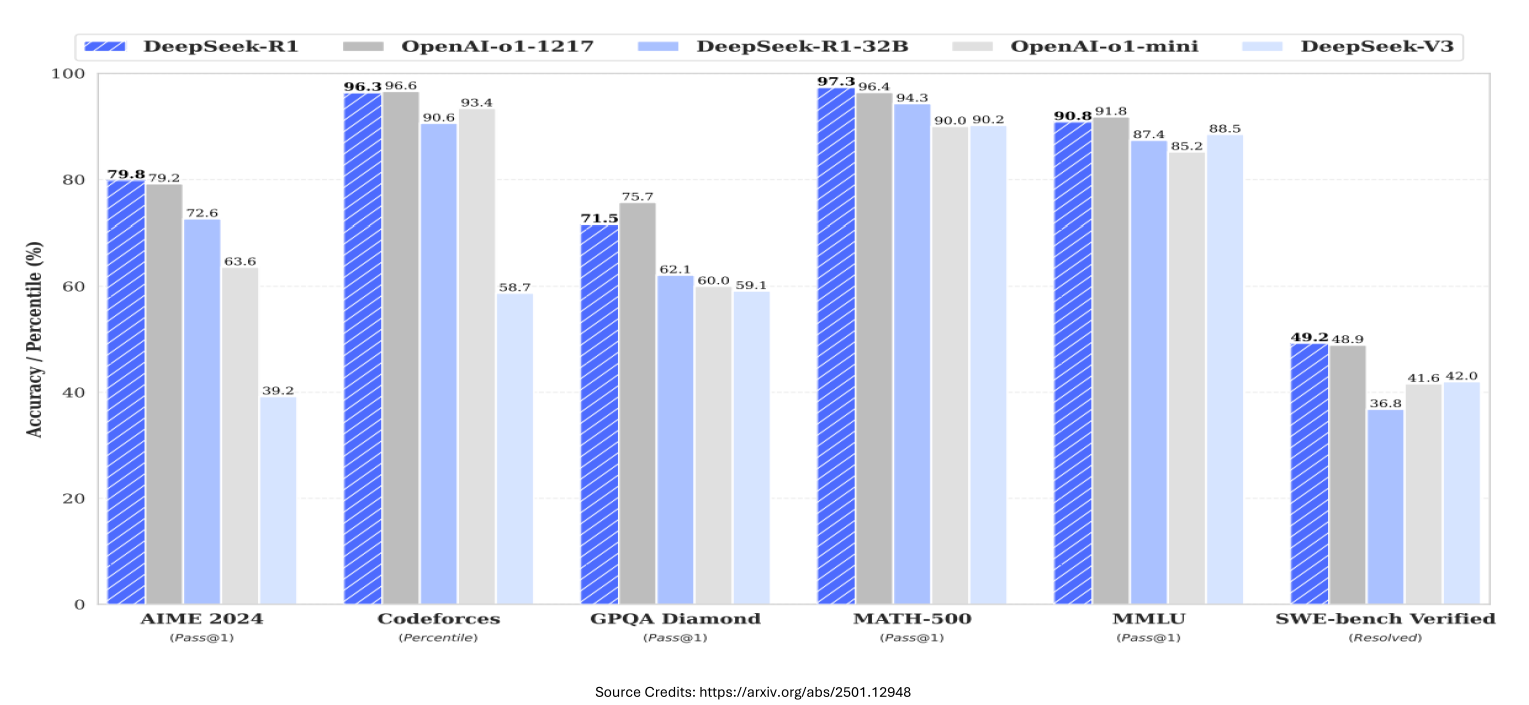
\includegraphics[width=\linewidth,keepaspectratio]{deepseek1}
		\end{center}

\end{frame}

%%%%%%%%%%%%%%%%%%%%%%%%%%%%%%%%%%%%%%%%%%%%%%%%%%%%%%%%%%%%%%%%%%%%%%%%%%%%%%%%%%
\begin{frame}[fragile]\frametitle{ Performance Comparison}
		\begin{center}
		{\textbf From DeepSeek-R1-Zero to DeepSeek-R1: DeepSeek-R1's Multistage Training Pipeline}
		\end{center}

\end{frame}

%%%%%%%%%%%%%%%%%%%%%%%%%%%%%%%%%%%%%%%%%%%%%%%%%%%%%%%%%%%%%%%%%%%%%%%%%%%%%%%%%%
\begin{frame}[fragile]{DeepSeek-R1}


    \begin{itemize}
        \item  Though DeepSeek-R1-Zero developed great reasoning capabilities, its 
language capabilities were not that great.
        \item  To solve these problems,  DeepSeek proposed a new multi-stage  
training process which resulted in DeepSeek-R1.
    \end{itemize}
\end{frame}



%%%%%%%%%%%%%%%%%%%%%%%%%%%%%%%%%%%%%%%%%%%%%%%%%%%%%%%%%%%%%%%%%%%%%%%%%%%%%%%%%%
\begin{frame}[fragile]{ Applications}

Real-World Applications of Reasoning Models

    \begin{itemize}
        \item   Scientific Research \& Problem Solving
		    \begin{itemize}
			\item   Assists in mathematical proofs, theorem validation.
			\item   Generates hypotheses in physics and chemistry.
			\end{itemize}
        \item   Automated Reasoning \& Decision Support
		    \begin{itemize}
			\item   Legal analysis (contract review, legal argument structuring).
			\item   Medical diagnosis assistance (differential diagnosis, symptom analysis).
			\end{itemize}			
        \item   Coding \& Debugging
		    \begin{itemize}
			\item   Code generation with logical step validation.
			\item   Error detection and reasoning-based fixes.
			\end{itemize}			
        \item   AI-Augmented Education
		    \begin{itemize}
			\item   Interactive tutors for logical reasoning and critical thinking.
			\item   Step-by-step guidance in STEM education.
			\end{itemize}			
    \end{itemize}
\end{frame}

%%%%%%%%%%%%%%%%%%%%%%%%%%%%%%%%%%%%%%%%%%%%%%%%%%%%%%%%%%%%%%%%%%%%%%%%%%%%%%%%%%
\begin{frame}[fragile]{ Trends}

Emerging Trends in Reasoning LLMs

    \begin{itemize}
        \item    Fine-tuning, reinforcement learning, and test-time scaling to 
optimize LLM performance. 
        \item    Long CoT (and inference-time scaling):  Using more compute at 
inference time—by generating a longer CoT— can allow users to 
dynamically improve a model’s reasoning capabilities.
        \item    Self-evolution through RL: Using large-scale RL training, the LLMs can 
execute complex reasoning strategies within their long CoT without 
explicitly being trained on this objective. 
        \item    Less human supervision: Reasoning models rely less on human 
supervision as compared to standard LLMs. Rewards during RL training 
are derived primarily from rules-based systems. 
        \item    Distillation: With large and powerful reasoning models, we can distil 
the capabilities of these models into smaller, dense models using 
simple strategies. 
    \end{itemize}
\end{frame}


%%%%%%%%%%%%%%%%%%%%%%%%%%%%%%%%%%%%%%%%%%%%%%%%%%%%%%%%%%%%%%%%%%%%%%%%%%%%%%%%%%
\begin{frame}[fragile]{ Challenges}

Open Challenges in Reasoning Models

    \begin{itemize}
        \item    Safety training for long CoT
        \item    Balance between general - reasoning capabilities
        \item    Optimal role of SFT in training reasoning models
        \item    Minimizing ``overthinking'' in long CoT
        \item    Efficient hosting of reasoning models
    \end{itemize}
\end{frame}


%%%%%%%%%%%%%%%%%%%%%%%%%%%%%%%%%%%%%%%%%%%%%%%%%%%%%%%%%%%%%%%%%%%%%%%%%%%%%%%%%%
\begin{frame}[fragile]{ Usages}

    \begin{itemize}
        \item chat.deepseek.com
		\item Ollama, LM Studio, Hugging Face
    \end{itemize}
\end{frame}

%%%%%%%%%%%%%%%%%%%%%%%%%%%%%%%%%%%%%%%%%%%%%%%%%%%%%%%%%%%%%%%%%%%%%%%%%%%%%%%%%%
\begin{frame}[fragile]\frametitle{ Summary}
		\begin{center}
		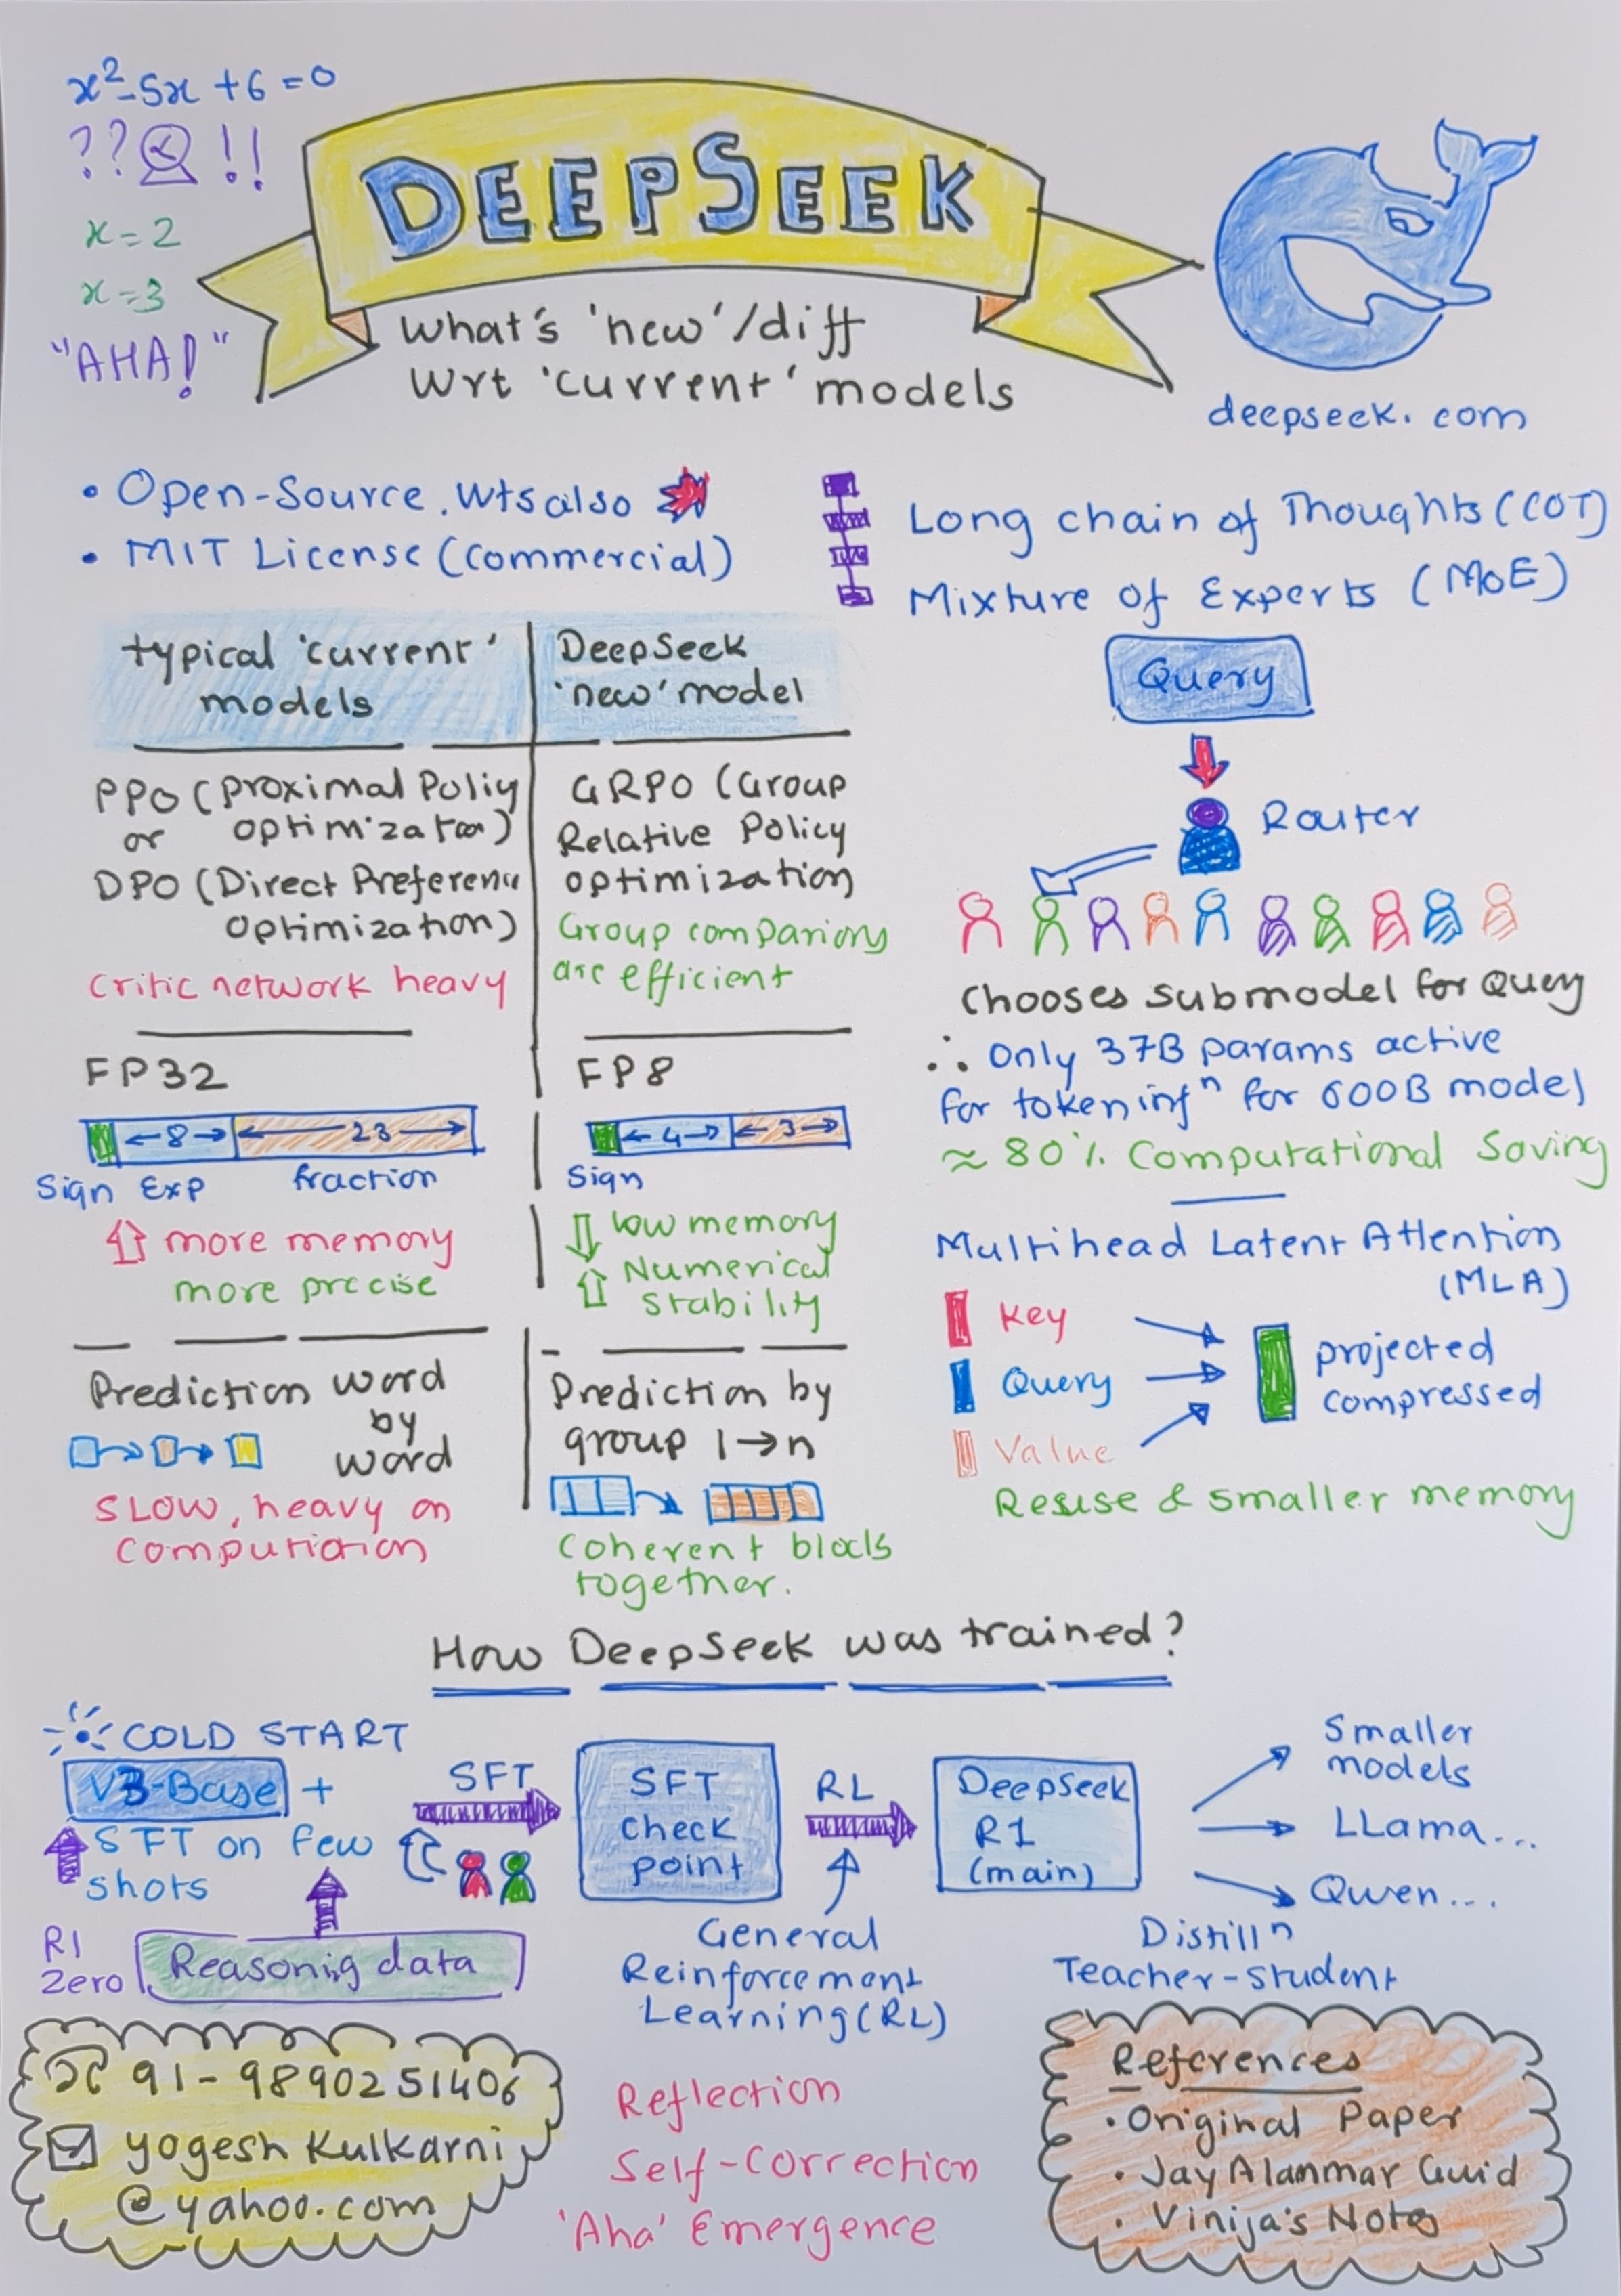
\includegraphics[width=0.45\linewidth,keepaspectratio]{DeepSeek_Sketchnote}
		\end{center}

\end{frame}


